\section{Uplifting 2D visual representations into 3D}
\label{sec:method_uplifting}

We now present a simple yet effective method for lifting 2D visual features into 3D using Gaussian Splatting, and discuss its relation with optimization-based techniques.

\subsection{Background on Gaussian Splatting}
\label{sec:background}

\myparagraph{Scene representation}
The Gaussian Splatting method consists in modeling a 3D scene as a set of~$n$ Gaussians densities $\Ncal_i$, each defined by a mean $\mu_i$ in $\mathbb{R}^3$, a covariance $\Sigma_i$ in $\mathbb{R}^{3\times 3}$, an opacity $\sigma_i$ in $(0,1)$, and a color function $c_i({d})$ that depends on the viewing direction $d$.
$d$ refers to the full camera pose, \ie its extrinsics and intrinsics.

A 2D frame at a given view is an image $\hat{I}_d$ rendered by projecting the 3D Gaussians onto a 2D plane, parametrized by the viewing direction $d$. This projection accounts for the opacity of the Gaussians and the order in which rays associated with each pixel pass through the densities.
More precisely, a pixel $p$ for a view $d$ is associated to an ordered set $\Scal_{{d},p}$ of Gaussians and its value is obtained by summing their contributions:
\vspace{-.07cm}
\begin{equation}\label{eq:render}
\hat{I}_{{d}}(p) = \sum_{i \in \Scal_{d,p}} c_i(d) w_{i}(d, p). 
\end{equation}
\vspace{-.07cm}
The above weights are obtained by $\alpha$-blending, \ie $w_{i}(d, p) = \alpha_{i}(d,p) \prod_{j\in \mathcal{S}_{d,p}, j<i} \left(1-\alpha_{j}(d,p)\right)$, 
where the Gaussian contributions $\alpha_{i}(d,p)$ are given by the product of the opacity $\sigma_i$ and the Gaussian density $\mathcal{N}_i$ projected onto the 2D plane at pixel position $p$.

\myparagraph{Scene optimization}
Let $I_1,\dots,I_m$ be a set of 2D frames from a 3D scene and $d_1,\dots,d_m$ the corresponding viewing directions. Gaussian Splatting optimizes the parameters involved in the scene rendering
function described in the previous section. This includes the means and covariances of the Gaussian densities, their opacities, and the color function parametrized by spherical harmonics. Denoting these parameters by $\theta$, the following reconstruction loss is used
\vspace{-.07cm}
 \begin{equation}
 \label{eq:gs-problem}
 \min_{\theta} \frac 1m \sum_{k=1}^m \mathcal{L}(I_k, \hat{I}_{d_k,\theta}),
 \end{equation}
\vspace{-.07cm}
where $\hat{I}_{d_k,\theta}$ is the frame of the scene rendered in the direction $d_k$ as in Eq.~(\ref{eq:render}), using the parameters $\theta$, and $\mathcal L$ is a combination of $\ell_1$ and SSIM loss functions~\citep{kerbl2023gaussiansplatting}.

\begin{figure*}[h!]
    \centering
    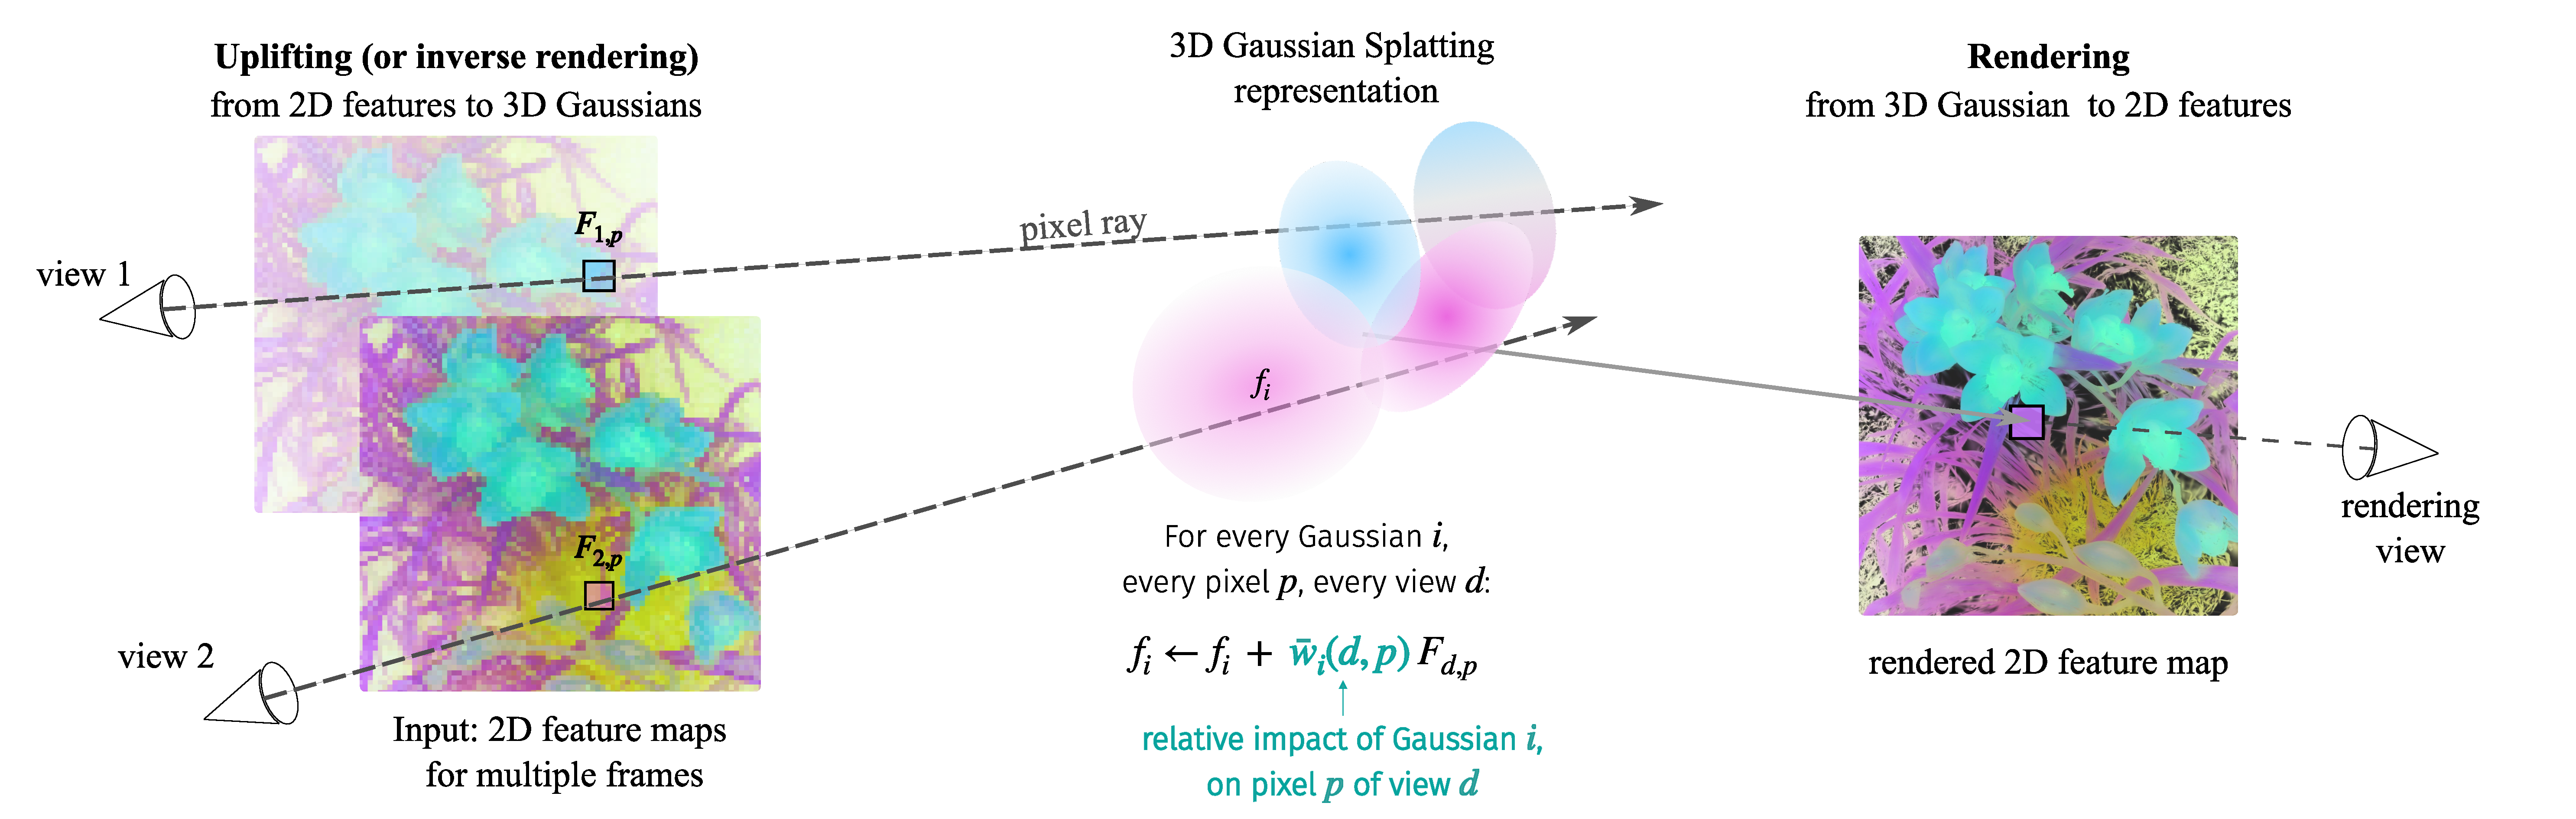
\includegraphics[width=.84\linewidth]{figures/fig2.pdf}
    \vspace{-0.2cm}
    \caption{\textbf{Illustration of uplifting and rendering.} In the uplifting phase, features ${\bf{f}}$ are created for each 3D Gaussian by aggregating coarse 2D features ${\bf F}$ over all viewing directions. For rendering, the 3D features ${\bf{f}}$ are projected on any given viewing direction as in regular Gaussian Splatting. The rendering weight $\bar{w}_{i}(d, p)$ represents the relative influence of the Gaussian $i$ on pixel $p$ (Eq.~(\ref{eq:uplifting})).} 
    \label{fig:uplift_render}
    \vspace{-.1cm}
    \vspace{-0.3cm}
\end{figure*}

\subsection{Uplifting 2D feature maps into 3D}
\label{sec:uplifting}

Given a 3D Gaussian Splatting scene representation, we propose a method to uplift any set of 2D features maps $\bf{F} = \{F_1,...,F_m\}$ associated to $m$ views into 3D. These features may be obtained from pretrained models~\cite{radford2021clip,oquab2024dinov2} or segmentation masks. The uplifted features ${\bf f}$ should allow for downstream 3D tasks, such as 3D segmentation, while being `faithful' when reprojected back in 2D.

\myparagraph{Uplifting with simple aggregation}
We construct uplifted features for each 3D Gaussian of the Gaussian Splatting scene as a weighted average of 2D features from all frames. 
Each 2D feature $F_{d,p}$ from a frame at a given viewing direction $d$ and pixel $p$ contributes to the feature $f_i$ by a factor proportional to the rendering weight $w_{i}(d, p)$, if the Gaussian $i$ belongs to the ordered set $\mathcal{S}_{d,p}$ associated to the view/pixel pair $(d,p)$. Denoting $\mathcal{S}_i = \{(d,p), i\in \mathcal{S}_{d,p}\}$ as the set of view/pixel pairs contributing to the feature $f_i$, the resulting features are defined as follows: 
\begin{equation}
    \label{eq:uplifting}
    f_i =  \!\! \sum_{(d,p) \in \mathcal{S}_i}  \! \bar{w}_{i}(d, p) F_{d,p},  ~~\text{}~~  \bar{w}_i(d,p) = \frac{w_{i}(d, p)}{\sum_{(d,p) \in \mathcal{S}_i} \! w_{i}(d, p)}.
\end{equation}
We can interpret this equation as a normalized version of the transposed rendering operation over the $m$ viewing directions. 
More precisely, the rendering of any view-independent collection of features ${\bf{f}} = (f_i)$ attached to the~$n$ Gaussians into the $m$ training frames can be represented as a linear operator $W$ acting on the collection $\bf{f}$ and returning a collection of 2D feature maps ${\bf{\hat{F}}} = (\hat{F}_{d,p})$, see Eq.~(\ref{eq:rendering}) below.
Here, non-zero entries of the matrix $W$ consists of all rendering weights $w_{i}(d, p)$ when $(d,p) \in \mathcal{S}_i$ is placed at row $(d,p)$ and column $i$, and $\mathbf{\hat{F}}$ is a 2D matrix containing all (flattened) 2D feature maps generated for all cameras poses, with $\mathbf{\hat{F}}_{d,p}$ the feature of pixel $p$ from view at direction $d$.
Similarly, the uplifting expression introduced in Eq.~(\ref{eq:uplifting}) can be expressed in terms of the transpose of $W$ and a diagonal matrix $D$ of size $m$ representing the normalization factor and whose diagonal elements are obtained by summing over the rows of $W$ as in Eq.~(\ref{eq:uplifting_matrix}) below:

\vspace{-.2cm}
\begin{minipage}{0.2\textwidth}
\[
\text{Rendering to $m$ frames}
\]
\begin{equation}
    {\bf \hat{F}} = W{\bf{f}},
\label{eq:rendering}
\end{equation}
\end{minipage}
\hfill
\begin{minipage}{0.2\textwidth}
\[
\text{Uplifting from $m$ frames}
\]
\begin{equation}
    {\bf f} = D^{-1}W^{\top}{\bf{F}}.
\label{eq:uplifting_matrix}
\end{equation}
\end{minipage}
\vspace{.3cm}

Note that $W$ and $D$ are never explicitly constructed. Instead, they are computed by calling the forward rendering function for Gaussian Splatting and replacing the color vectors by the feature vectors (see Fig.~\ref{fig:uplift_render}). All these operations are performed within the CUDA rendering process.

\myparagraph{Connection with optimization-based inverse rendering}  
An alternative approach to uplifting 2D features ${\bf F}$ is to minimize a reconstruction objective $\mathcal{L}({\bf f})$, where the goal is to find uplifted features~${\bf f}$ whose rendering closely matches the original 2D features ${\bf F}$ \citep{tschernezki2022n3f, kerr2023lerf, zuo2024fmgs}. A natural choice is to minimize the mean squared error between the 2D features~${\bf F}$ and the rendered ones ${\bf \hat{F}}$ as defined by Eq.~(\ref{eq:rendering}):
\begin{align}
\min_{{\bf f}} \mathcal{L}({\bf f}) := \frac{1}{2}\Vert {\bf F} - W{\bf f} \Vert^2.
\label{eq:reconstruction_loss}
\end{align}
Such an approach requires an optimization procedure which is costly compared to our proposed uplifting method. Nevertheless, it is possible to interpret the proposed uplifting scheme in Eq.~(\ref{eq:uplifting_matrix}) as a single pre-conditioned gradient descent step on the reconstruction objective, starting from a~${\bf 0}$~feature, \emph{i.e.}, ${\bf f}= -D^{-1}\nabla \mathcal{L}({\bf 0})$. In practice, we found that performing more iterations on the objective $\mathcal{L}({\bf f})$ did not improve the quality of the features, thus suggesting that the computationally cheaper scheme in Eq.~(\ref{eq:uplifting_matrix}) is already an effective approach to uplifting.

\myparagraph{Gaussian filtering}
The normalization term $\beta_i = \sum_{d,p\in \mathcal{S}_i} w_{i}(d, p)$ serves as an estimator of the relative importance of each Gaussian in the scene. Therefore, it can be used as a criterion to prune the set of Gaussians for memory efficiency. In our experiments, we filter out half of the Gaussians based on $\beta_i$ and observe no qualitative nor quantitative degradation of the results. This approach is inspired by prior work on efficient Gaussian Splatting representation such as proposed by~\cite{fan2023lightgaussian} that also prunes Gaussians based on their contribution to each pixel in the training frames.  

\subsection{Enriching features by graph diffusion}
\label{sec:diffusion}
DINOv2 features have shown remarkable performance on semantic segmentation with simple linear probing~\citep{oquab2024dinov2}, making them 
a good candidate to enrich features that lack such a property, such as those from CLIP~\citep{wysoczanska2023clipdino,zuo2024fmgs,liu2023weakly}. 
Inspired by spectral clustering techniques~\citep{shi2000normalized,kondor2002diffusion,belkin2001laplacian} and manifold denoising~\citep{hein2006manifold}, 
we propose to \textit{diffuse} features that have been uplifted to 3D. This process aims to align semantic features with the scene layout and object boundaries implied by DINOv2.
In contrast to prior work, we perform this landscaping with DINOv2 directly in the 3D scene, thereby taking 3D geometry into account as well.

\myparagraph{Graph construction}
We construct a graph whose nodes are the $n$ 3D Gaussians and edges, represented by a matrix $A$ of size $n\times n$, are based on 3D Euclidean geometry between the nodes and the similarity between their DINOv2 features. More precisely, we extract the $k$ nearest neighbors $\mathcal{N}(i)$ for each node $i$, as measured by the Euclidean distance between the centers of the 3D Gaussians. 
Two nodes $i$ and $j$ in the graph are linked by an edge if $i \in \mathcal{N}(j)$ or $j \in \mathcal{N}(i)$, and the edge is assigned the following weight:
\vspace{-.07cm}
\begin{equation}
\label{eq:edges}
A_{ij} = S_f(f_i, f_j) \, P(f_i)^{\frac 12}P(f_j)^{\frac 12}, 
\vspace{-.07cm}
\end{equation}
with $S_f(f_i,f_j)$ a local similarity between features $f_i$ and $f_j$, typically defined as a RBF kernel. For tasks requiring diffusion to be confined to a specific object instance, we prevent leakage into the background by introducing a node-wise unary regularization term $P(f_i)$ which quantifies the similarity between the node feature $f_i$ and the features of the object of interest. Details on $S_f$ and $P$ are provided in the supplementary (Sec.~\ref{sec:appendix-diffusion}).

\myparagraph{Diffusion on the graph}  
Given initial 3D features $g_0$ in $\mathbb{R}^n$, which we aim to improve by using information encoded in $A$ (3D geometry and DINOv2 similarities), we perform $T$ diffusion steps to construct a sequence of diffused features $(g_t)_{1\leq t \leq T}$  defined as follows:
\vspace{-.07cm}
\begin{equation}
g_{t+1} = A\tilde{g}_{t}, \quad \tilde{g}_{t} = {g_t}/{\|g_t\|_2},
\label{eq:diffusion}
\vspace{-.07cm}
\end{equation}
This can be seen as performing a few steps of the power method, projecting $g_0$ into the dominant eigenspace of~$A$. Depending on the task, $g_0$ may represent generic features or task-specific features such as 3D segmentation masks.
\vspace{-.05cm}